\section{Results and Discussion}

We organize our results in three parts. 
First, we present a broad exploration of different license types, highlighting 
their prevalence, retention, and general trends.
Next, we detail the regression analysis that examines how the choice of license 
relates to project performance. 
Finally, we focus on the phenomenon of license switching by analyzing performance
metrics before and after a change from permissive to restrictive (or vice versa).

\subsection{The Types and Prevalence of Licenses Across the OSS Landscape}

\subsubsection{Our Findings}

We first counted the total number of projects that had at least one occurrence 
of any license during their lifetime.
We then identified the top 20 most used licenses, 
as shown in Figure~\ref{fig:dis1}.

Out of the 131,171,379 projects indexed by WoC, 22,281,342 projects had at 
least one license committed to their project at some point in their lifetime.
However, when examining the latest version of these projects, 
this number drops to 20,110,256 projects.

When interpreting the numbers shown in these figures, it is important to note 
that the sum of these numbers exceeds the total number of projects with a license.
This discrepancy arises because some projects have multiple licenses and 
are therefore counted in several categories.

\begin{figure*}[t]
\centering
    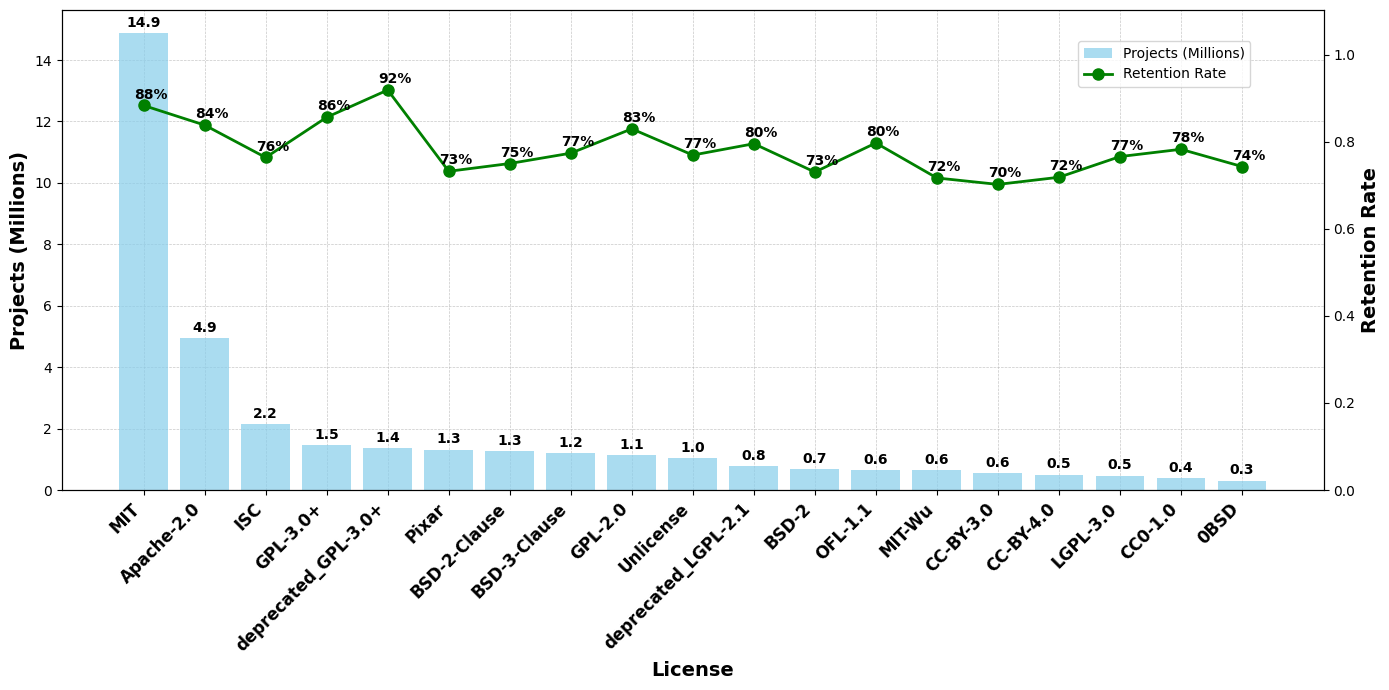
\includegraphics[width=\textwidth]{figures/dis1.png}
    \caption{The distribution and retention rates of the most used licenses.}
    \label{fig:dis1}
    \Description{The distribution and retention rates of the most used licenses.}
\end{figure*}

To calculate the retention rate for each license, we determined the number of 
projects that still had the license in their latest state and divided this number 
by the total number of projects that had ever used the license.
This retention rate indicates the proportion of projects that continue to use 
the license over time, and it is also displayed in Figure~\ref{fig:dis1}.

As shown in the figure, the MIT license is the most prominent, followed
by the Apache 2.0 and ISC licenses.
Notably, per H1b, the deprecated GPL 3 license (with strong
copyleft provisions) exhibits the highest retention rate.
In contrast, the Creative Commons 3 license (CC-BY-3.0) 
shows the lowest retention rate among the top 20 most used licenses.

\begin{figure}[t]
\centering
    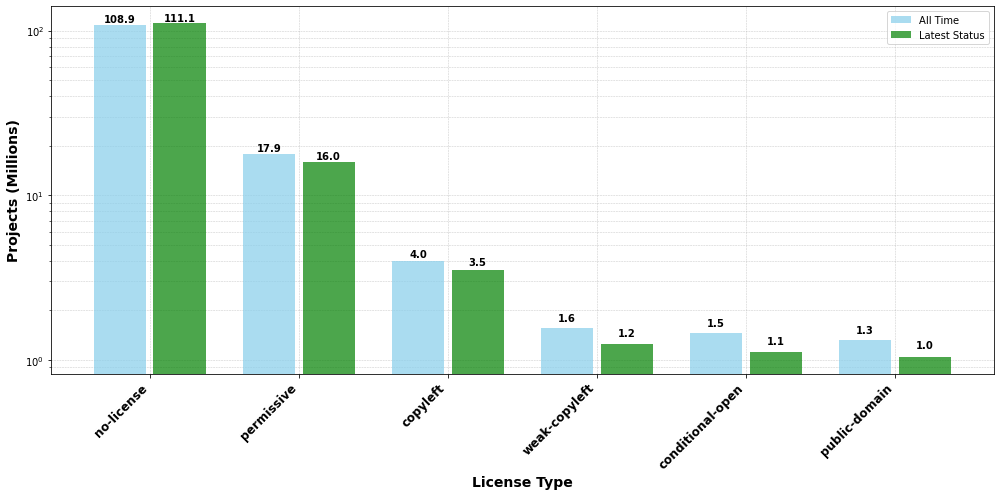
\includegraphics[width=\linewidth]{figures/dis3.png}
    \caption{The distribution of license types across projects.}
    \label{fig:dis3}
    \Description{The distribution of license types across projects.}
\end{figure}

We also analyze the distribution of projects according to their license types.
Initially, we consider the distribution across the entire project history, 
meaning that if a project adopted a license at any point and later removed it, 
it is still counted as having that license.
Next, we determine the distribution based on the most recent status of 
each project.

Figure~\ref{fig:dis3} shows that ``conditional-open'', ``weak-copyleft'', 
and ``public-domain'' license types have the lowest
retention, with approximately a quarter of the projects that ever had 
such license changing it by their latest version.
For comparison, only approximately 8\% of ``copyleft'' licenses were changed, 
which is consistent with our theory (H1b) that ideology-related license choice should be most ``sticky''. 


We also analyze the proportion of adopted licenses at each point in time, 
categorized by license type, to identify trends in licensing preferences over 
time. This allows us to observe shifts in the adoption of different 
licenses and assess whether certain license types have gained or declined 
in popularity. By tracking these proportions longitudinally, we can better 
understand how licensing choices evolve and whether external factors, such 
as regulatory changes or community norms, influence these trends.
Th results are shown in Figure~\ref{fig:proportion}.

\begin{figure}[t]
    \centering
    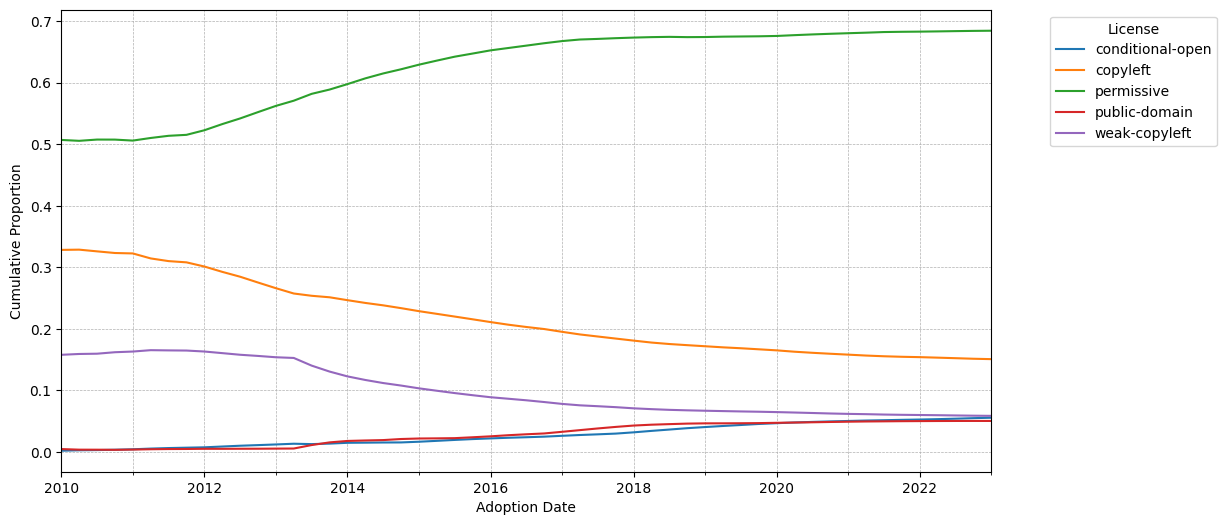
\includegraphics[width=\linewidth]{figures/proportion.png}
    \caption{Proportion of license type over time}
    \label{fig:proportion}
    \Description{Proportion of license type over time}
\end{figure}

Looking at the trends we clearly see that although copyleft licenses
may be the most sticky, the tendency to adopt these licenses has decreased
over time.

\subsubsection{Comparison with Literature}

Table~\ref{tab:res1a} provides a comparison between the results in the 
literature and our study, highlighting substantial differences primarily 
due to variations in scope, methodology, and dataset size 
(see Table~\ref{tbl:litRev}).

\begin{table*}[t]
\centering
\caption{Comparison between our results and the literature.}
\label{tab:res1a}
% \resizebox{0.99\linewidth}{!}{
\begin{tabular}{lrr|rrrrr}
    \toprule
    & \textbf{Projects} & \textbf{No License} & \textbf{Copyleft} & \textbf{Weak} & \textbf{Conditional} & \textbf{Permissive} & \textbf{Public} \\
    & & & & \textbf{Copyleft} & \textbf{Open} & & \textbf{Domain} \\
    \midrule
    \cite{wu2024large} & 3,474,778 & 21.12\% & 5.72\% & 5.12\% & - & 89.16\% & - \\
    \cite{cui2023empirical} & 16,341 & 10.51\% & 11.32\% & 0.97\% & - & 87.71\% & - \\
    \textbf{This Study} & 131,171,379 & 83.01\% & 15.35\% & 5.26\% & 4.82\% & 70.18\% & 4.39\% \\
    \bottomrule
\end{tabular}
\end{table*}


A key methodological difference between our study and \citet{wu2024large} lies in the treatment of data points.
\citet{wu2024large} considered each version of a package as a separate data point, 
resulting in 46.59 million data points from 3.47 million projects.
This approach could introduce bias by overrepresenting projects with many
versions, potentially skewing observed trends in licensing.
Conversely, our study treated each project as a single data point, providing 
a more balanced view of the open source ecosystem without overemphasizing 
projects with frequent updates.

The focus of the \citet{wu2024large} study on only five package managers might explain 
the significant discrepancy in the percentage of projects without a license.
Their study reported that 21.12\% of projects lacked a license,\footnote{
Since the paper provides these percentages by package manager, we calculated the 
overall percentage by taking a weighted average based on the number of 
projects per package manager.} 
whereas our study found a much higher percentage of 83.01\%.
On the other hand, \citet{cui2023empirical} reported that only 10.51\% of
projects were unlicensed.
The difference with \citet{wu2024large} likely stems from the fact that the
package managers they examined are associated with more mature and 
well-maintained projects, which are more likely to have defined licenses.
Additionally, \citet{cui2023empirical} filtered their data to include 
only projects with over 1,000 stars, which might explain why the 
percentage of unlicensed projects is so low\footnote{
These could also be influenced by the differences between OSS projects
and publicly available projects as was explained in the introduction.}.
In contrast, our broader dataset includes a wide variety of projects, many 
of which may be less mature or less formally governed, leading to a higher incidence of unlicensed projects.

The analysis of copyleft versus permissive licenses further reflects 
the differences in scope.
\citet{wu2024large} found a dominance of permissive licenses, with much 
lower percentages for copyleft and weak copyleft licenses.
However, our study, covering all programming languages, reveals a more 
diverse licensing landscape, with a lower percentage of permissive licenses
and higher percentages of copyleft licenses.
This suggests that by focusing on just five package managers, \citet{wu2024large}
might underrepresent broader licensing trends, particularly the prevalence 
of copyleft licenses across the global open source ecosystem.

\begin{figure}[t]
\begin{tcolorbox}[colback=gray!5!white, colframe=gray!70!black, title=Key Findings]
\small
\begin{enumerate}[leftmargin=4mm]
    \item Overall, 83\% of the projects in the dataset lack a formal license, which is significantly higher than the figures reported in previous studies.
    \item The MIT license is the most widely used license,
      accounting for 65\% of all licensed projects and 10\% of all
      OSS projects.
    \item Despite the overall preference for permissive licenses,
      copyleft licenses such as GPL exhibit strong retention rates
      as suggested by H1b.
    \item The differences in license usage reported in our study compared 
    to previous literature highlight the importance of dataset scope 
    and methodology when assessing the prevalence of licenses in OSS projects.
\end{enumerate}
\end{tcolorbox}
\Description{Key Findings}
\end{figure}

\subsubsection{Implications}

The analysis of public repository licensing reveals that 83\% of projects lack a
formal license, posing significant legal risks and discouraging
innovation by preventing responsible actors from reusing unlicensed code. 
This highlights the need for developers to prioritize licensing to set 
clear terms of use.
Our findings challenge previous studies, which often underestimate the 
prevalence of unlicensed projects by focusing on mature ones, missing 
the broader risks of software reuse.

Even though many of these unlicensed projects may seem trivial and 
technically not OSS, their 
public availability still creates legal ambiguity and poses a risk 
of license noncompliance, especially when combined with the lack of 
thorough legal review in many downstream projects.
\citet{jahanshahi2024beyond} demonstrated that in the context of 
copy-based reuse, nearly 18\% of reused artifacts originated from 
very small projects,\footnote{
Projects with no stars and fewer than 10 commits.
} while large projects\footnote{
Projects with more than 10 stars and 100 commits.
} accounted for only 32\% of reused artifacts.
This highlights the importance of addressing the issue of unlicensed code within the OSS ecosystem.

Among projects that are licensed, the MIT license is the most prevalent, 
reflecting a historic preference for permissive licenses that facilitate 
broad adoption and collaboration.
However, the continued use of copyleft licenses like the GPL
(which was popular decades ago)
demonstrates that many developers are committed to preserving the
open nature of derivative works.

\subsection{The Impact of License Choice on Project Characteristics}

\subsubsection{Our Findings}

Now we turn to the results of our regression model discussed in Section~\ref{sec:reg}.
The basic statistics of the response and control variables, including the 
5th percentile, median, mean, and 95th percentile for the numeric variables, 
as well as the counts of different levels for the factor variables, 
are presented in Table~\ref{tbl:stat-l}.

\begin{table*}[t]
\centering
\caption{License type model - descriptive statistics.}
\resizebox{0.99\textwidth}{!}{
\begin{tabular}{cllcccc}
  \toprule
  & \textbf{Variable} & \textbf{Description} & & \textbf{Statistics} & & \\ 
  \midrule
  \midrule
  \multirow{9}{*}{\rotatebox{90}{\textbf{Response}}} 
  & & & \textbf{5\%} & \textbf{Median} & \textbf{Mean} & \textbf{95\%} \\ 
  & LatestCommit & Time since the latest commit & 04/30/2011 & 02/17/2020 & 03/15/2019 & 04/28/2023 \\
  & Active Month & Number of active months & 1 & 7 & 21.65 & 88 \\
  & Burstiness & (Latest - Earliest) / Active months & 0 & 1 & 1.87 & 6.37 \\
  & Authors & Number of authors & 1 & 2 & 23.31 & 56 \\
  & Commits & Number of commits & 2 & 155 & 2,982.63 & 5,770 \\
  & UpProjects & Number of upstream projects & 1 & 44 & 209.21 & 875 \\
  & DownProjects & Number of downstream projects & 0 & 12 & 1,831.07 & 2,342 \\ 
  & Files & Number of files & 5 & 1,820 & 17,295.57 & 59,939.60 \\ 
  & Blobs & Number of blobs & 15 & 5,616 & 19,952.34 & 51,076 \\
  \midrule
  \multirow{5}{*}{\rotatebox{90}{\textbf{Control}}} 
  & EarliestCommit & Time since the earliest commit & 05/08/2006 & 07/05/2017 & 01/31/2016 & 11/23/2021 \\
  & AdoptDelay & Earliest commit to license adoption (days) & 0 & 0 & 133 & 751 \\ 
  \multicolumn{6}{c}{\dotfill} \\
  & Language & \hspace{-0.2cm}JavaScript \hspace{1.15cm} C/C++ \hspace{1.1cm} Python & Java & PHP & Ruby & (Remaining) \\ 
  & Counts (\%) & \hspace{-0.6cm}221,588 (38.72\%) \hspace{0.1cm} 82,551 (14.43\%) \hspace{0.1cm} 53,468 (9.34\%) & 50,372 (8.80\%) & 44,952 (7.86\%) & 18,592 (3.25\%) & 100,650 (17.59\%) \\ 
  \midrule
  & License & \hspace{0.0cm}No License \hspace{1.5cm} Permissive & \hspace{-1.3cm} Copyleft & Weak Copyleft & Conditional Open & Public Domain \\ 
  & Counts (\%) & \hspace{-0.35cm} 263,974 (46.13\%) \hspace{0.7cm} 148,320 (25.92\%) & \hspace{-1.2cm} 60,925 (10.65\%) & 43,143 (7.54\%) & 30,933 (5.41\%) & 24,878 (4.35\%) \\
  \bottomrule
\end{tabular}}
\label{tbl:stat-l}
\end{table*}

Given that we have multiple response variables, the model provides a distinct set of coefficients for each outcome.
Each set of coefficients indicates the influence of the predictor variables 
on the probability of the response variable assuming that there might 
be correlation between response variables.

For categorical variables, we employed sum contrasts, also known as effect 
coding, where each level of the predictor variable is compared to the 
overall mean of all levels.
This approach is particularly advantageous in models where the goal is to 
compare each category to the overall mean rather than to a specific 
reference category, as it offers a more symmetric interpretation of the effects.
In the sum contrast method, the sum of the coefficients for all levels, including the intercept, must equal zero.
We also include the interaction term between language and license in the model.

Furthermore, in interpreting the earliest and latest commit times, it is important to emphasize that the predictors used in the model represent the time elapsed since those commits.
This means that a higher value for the earliest commit indicates that the commit occurred further in the past (i.e., the project is older), and a lower value indicates a more recent commit.

Table~\ref{tbl:anova-l}) shows Type III MANOVA Tests with Pillai test statistic
for the fitted model. 
The results show that the p-values for all the predictors are close to zero, 
indicating that each predictor significantly improves our model's fit.

\begin{table}[t]
\centering
\caption{License choice model - Type III MANOVA Tests: Pillai test statistic}
% \resizebox{\linewidth}{!}{
\begin{tabular}{lccc}
    \toprule
    \textbf{Variable} & \textbf{DF} & \textbf{Test Stat} & \textbf{p.value} \\ 
    \midrule
    (Intercept) & 1 & 0.29263 & \cellcolor{lightgreen}$<2\times10^{-16}$ \\
    License & 5 & 0.04443 & \cellcolor{lightgreen}$<2\times10^{-16}$ \\
    Language & 11 & 0.09268 & \cellcolor{lightgreen}$<2\times10^{-16}$ \\
    EarliestCommit & 1 & 0.60320 & \cellcolor{lightgreen}$<2\times10^{-16}$ \\
    Delay & 1 & 0.11327 & \cellcolor{lightgreen}$<2\times10^{-16}$ \\
    License:Language & 55 & 0.07032 & \cellcolor{lightgreen}$<2\times10^{-16}$ \\
    \bottomrule
\end{tabular}
\label{tbl:anova-l}
\end{table}


\begin{figure*}[t]
    \centering
    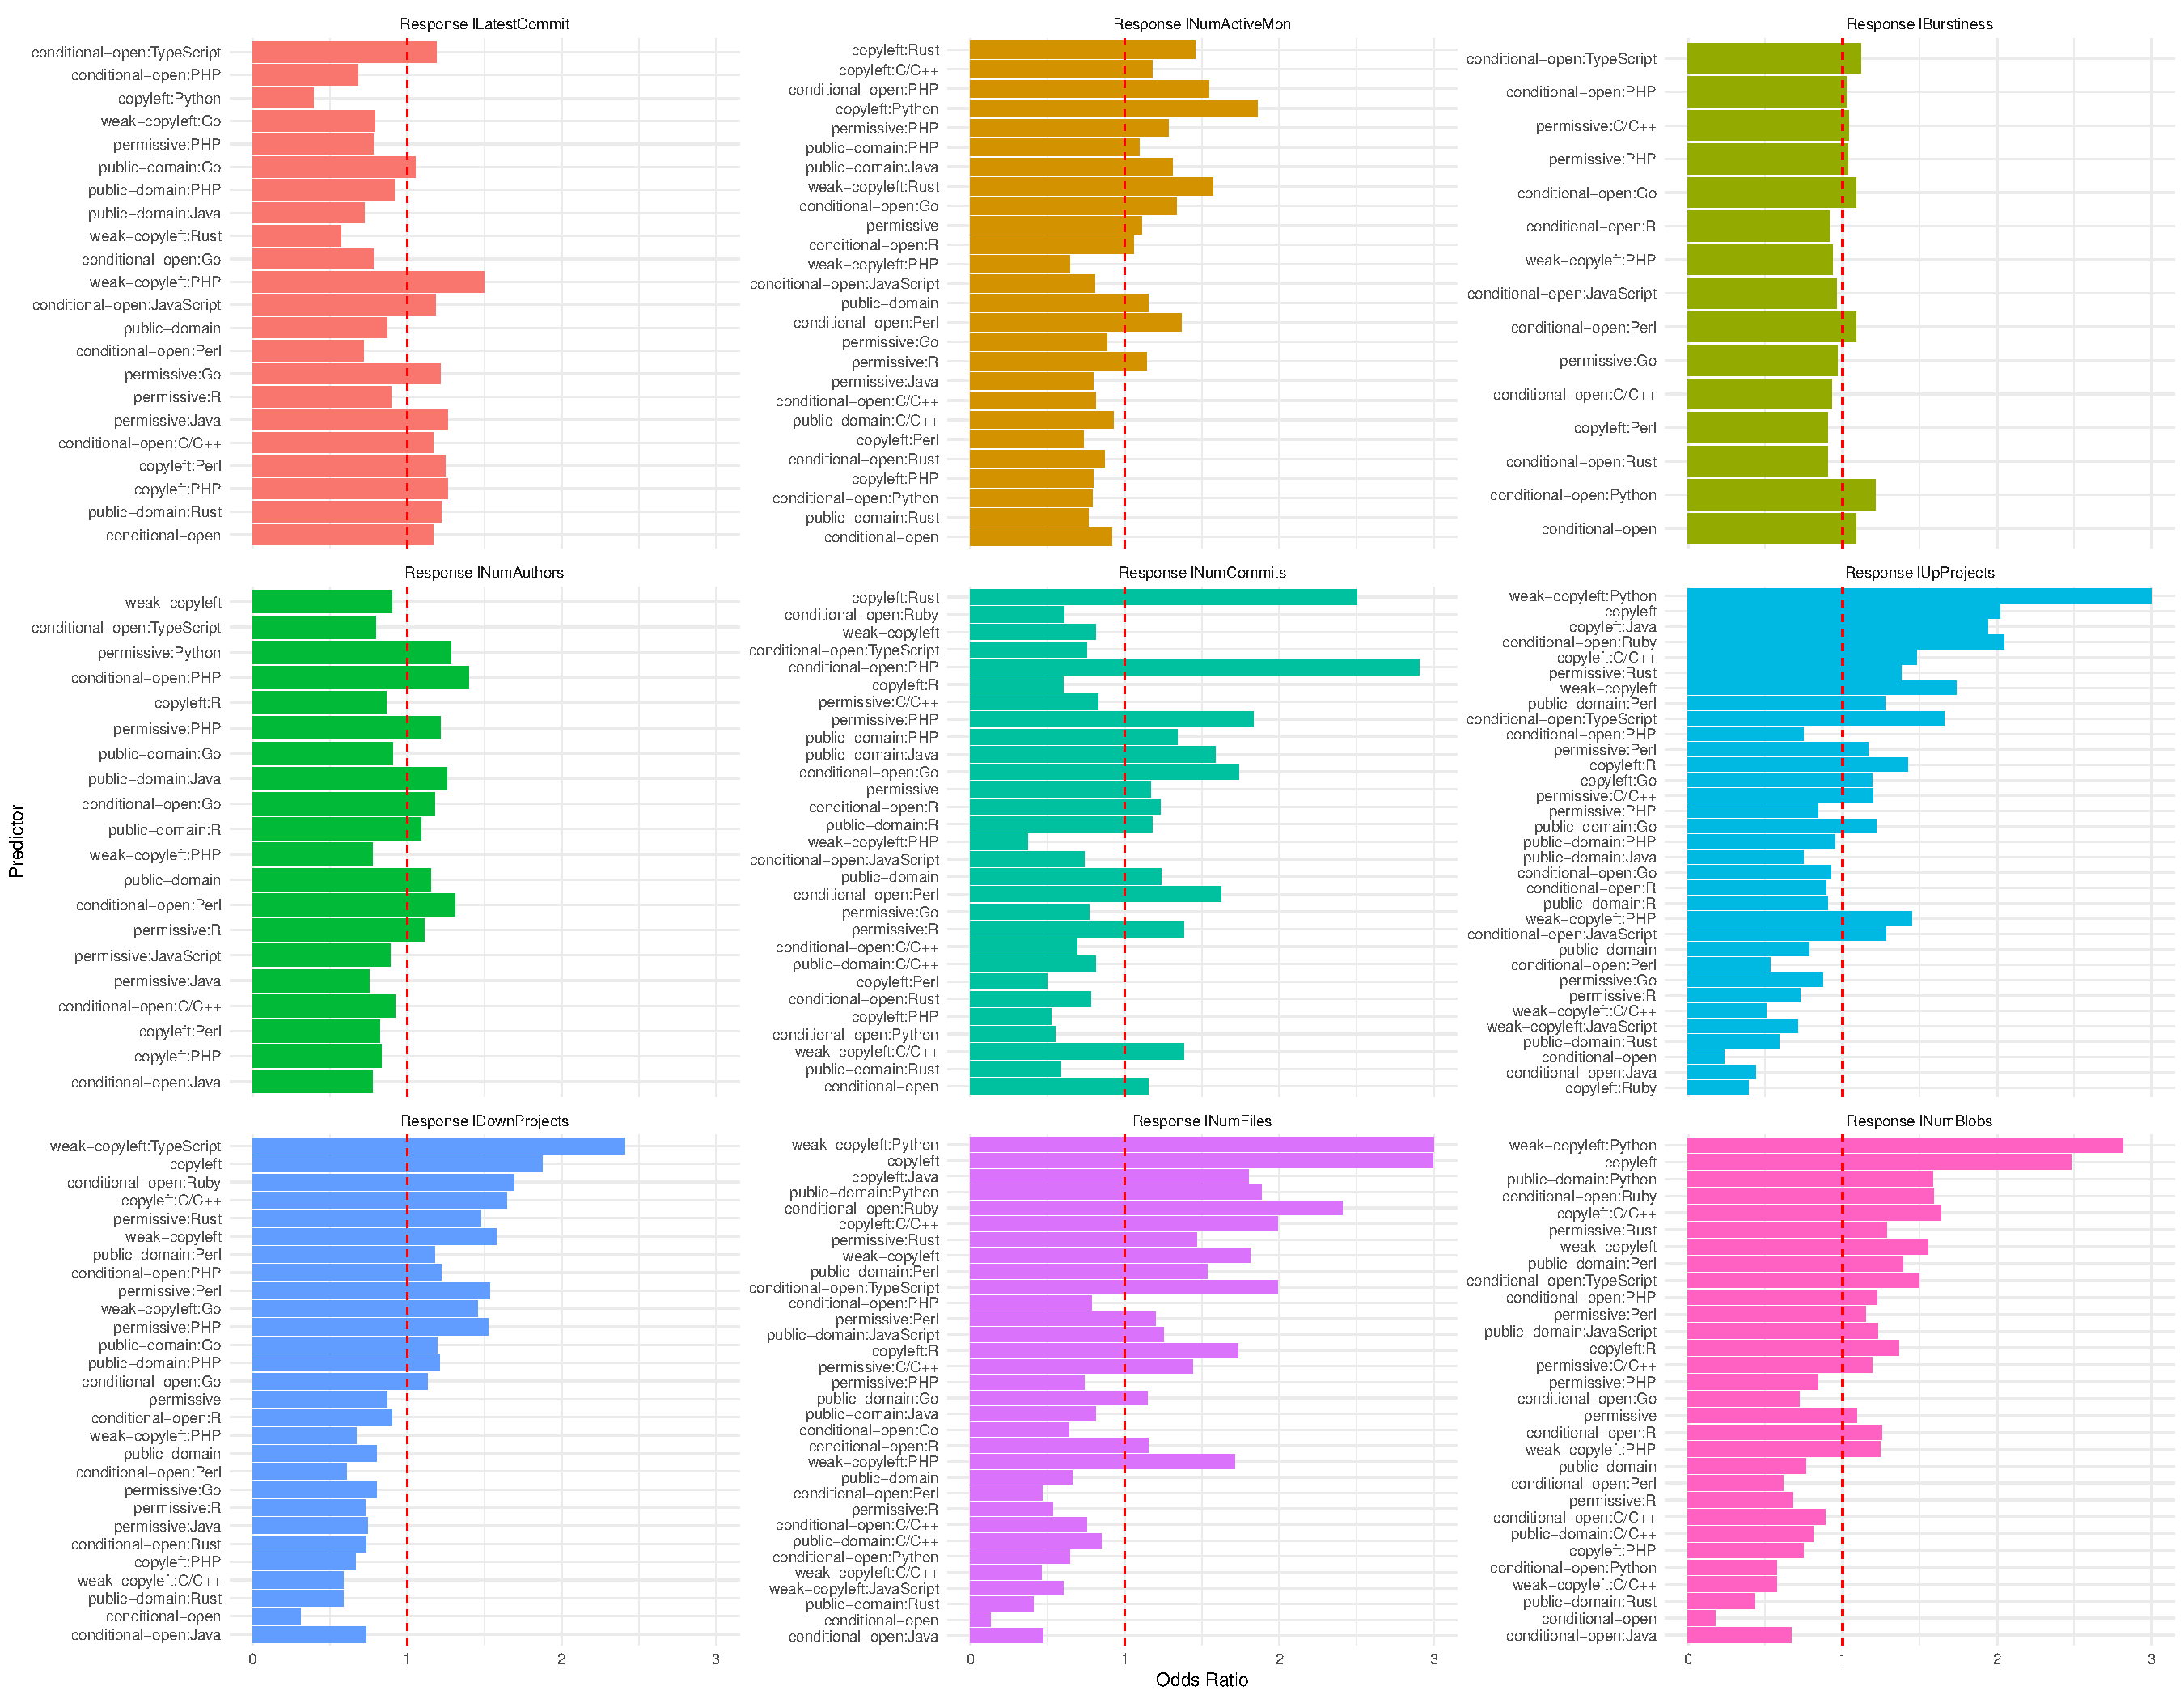
\includegraphics[width=\linewidth]{figures/odds_ratio_plot.pdf}
    \caption{License choice model - odds ratios}
    \label{fig:probs}
    \Description{License model - odds ratios}
\end{figure*}


%%%%%%%%%%%%%%%%%%%%% H1 %%%%%%%%%%%%%%%%%%%%%



%%%%%%%%%%%%%%%%%%%%% H2 %%%%%%%%%%%%%%%%%%%%%

Our analysis shows significant variation in licensing preferences
across programming languages, reflecting the community culture and
technical norms associated with each language (as predicted by H2a).
JavaScript, Ruby, TypeScript, and Go exhibit a strong preference for
permissive licenses (e.g., MIT, Apache), likely due to their
dominant role in web development and collaborative environments or
because these communities started from using such licenses. 
Conversely, Perl, R, and C/C++ favor copyleft licenses (e.g., GPL),
aligning with their historical ties to the early days of open-source movement when
copy-left licenses were more common (H2a) (see Figure~\ref{fig:proportion}).

As the number of forks increases, projects show a clear shift toward
permissive licenses, with the likelihood rising from 55.26\% to
60.10\%, while the adoption of copyleft and conditional licenses
declines slightly. 
This supports the H2b that projects with more forks, perceived as valuable by the community, tend to prioritize collaboration and reuse by favoring permissive licenses.

For downstream projects, the likelihood of selecting conditional open,
public domain, and weak copyleft licenses increases modestly. 
Meanwhile, both permissive and strong copyleft licenses see a 
slight decline. This suggests that developers with more downstream 
interactions are leaning toward less restrictive licenses, supporting H2b.
This is 
reflected by the decrease in strong copyleft and increase in weak 
copyleft, possibly driven by motivations similar to Hypothesis H1c. 
Additionally, the increase in public domain licensing and decline 
in permissive licenses may also reflect a shift toward even 
fewer restrictions.

%%%%%%%%%%%%%%%%%%%%% H3 %%%%%%%%%%%%%%%%%%%%%

% delay
As the delay in adopting a license increases (from 1 to 12 months),
projects show a slight increase in the likelihood of selecting
conditional open, public domain, and weak copyleft licenses. 
Meanwhile, the probability of choosing a permissive license
decreases.
This suggests that longer delays allow more time for legal and
community considerations, leaning towards less known licenses.
The probability of selecting a copyleft license remains stable,
suggesting it is less influenced by the timing of the decision. 
Overall, our hypothesis H3a that more delay translates in less common
license is confirmed, as the permissive and copyleft licenses are
the most used (known) licenses in OSS. 

%%%%%%%%%%%%%%%%%%%%% H4 %%%%%%%%%%%%%%%%%%%%%

As project activity increases, reflected by the number of commits, there is a rise in the adoption of copyleft and permissive licenses, with the probability of conditional open and public domain licenses decreasing.
This suggests that projects with more frequent development cycles
may lean toward either protection via copyleft or flexibility via
permissive licenses. While this partially supports H4a, that too permissive 
licenses (e.g. public domain) will not be favored, the increase in strong copyleft
contradicts our hypothesis.

For larger projects, as measured by the number of files, there is a 
notable increase in weak copyleft licenses, while permissive licenses 
see a sharp decrease. This suggests that as complexity grows, 
developers may prefer licenses that offer more control and protection, 
aligning with the hypothesis that larger, modular projects balance 
reuse with intellectual property concerns, supporting H4b. 
In contrast, conditional open, public domain, and strong copyleft 
licenses show only modest increases.

Older projects, as indicated by the time since the earliest commit,
show a preference for copyleft licenses, while newer projects are
more likely to adopt permissive or conditional open licenses (H4c). 
This reflects the hypothesis that mature projects may seek
sustainability and protection, while newer projects prioritize rapid
contributions or, that older projects, at theirs start, were relatively more
exposed to copyleft licenses (H2a, see Figure~\ref{fig:proportion}).



Inactive projects, marked by longer time since the latest commit,
show slight increases in conditional open, copyleft, and weak
copyleft licenses, while permissive and public domain licenses
decrease. 
This suggests that flexible licenses may correlate with continued
activity, while more restrictive licenses become prevalent as
projects age. This could also be the result of older projects
leaning toward more restrictive licenses.

In bursty projects (those with fluctuating activity), both
permissive and copyleft licenses increase slightly, reflecting the
dual need for flexibility and protection.
This aligns with the hypothesis that bursty projects may prefer
licenses that are more popular and used in many other projects (H4d).

\begin{comment}
As theorised, software project licensing preferences are influenced by
various factors, including the number of commits, files, core
authors, female authors, forks, downstream projects, project age,
and activity levels.

As commits increase, projects tend to favor copyleft and permissive licenses, while conditional open, public domain, and weak copyleft licenses become less common.
In contrast, projects with more files shift away from permissive licenses toward conditional open, public domain, and weak copyleft licenses, with copyleft licenses remaining stable.

The number of core authors slightly reduces the likelihood of adopting conditional open, copyleft, and public domain licenses, while permissive licenses gain a slight preference.
Projects with more female authors tend to adopt conditional open and public domain licenses more frequently, with a corresponding decline in copyleft and permissive licenses.

As forks increase, there is a clear preference for permissive licenses, while conditional open, copyleft, public domain, and weak copyleft licenses decrease.
Similarly, as downstream projects grow, developers lean toward licenses with more specific conditions for control and protection.

Over time, older and inactive projects shift from permissive and conditional licenses to copyleft and weak copyleft, while projects in bursty development environments slightly favor permissive licenses for their simplicity.

Ultimately, licensing choices are shaped by cultural, historical, and practical factors.
Permissive licenses dominate many programming languages due to their flexibility, while copyleft licenses are preferred in communities that prioritize long-term software freedom.
Language-specific use cases and historical context also play a key role in shaping these preferences.
\end{comment}

\subsubsection{Comparison with Literature}

Table~\ref{tab:res1b} provides a comparison between the results in the literature and our study, highlighting substantial differences primarily due to variations in scope and sampling strategy.

\begin{table*}[t]
\centering
\caption{Comparison with literature}
\label{tab:res1b}
\resizebox{0.99\textwidth}{!}{
\begin{tabular}{lllr|rrrrr}
    \toprule
    \multirow{2}{*}{\textbf{Language}} & \multirow{2}{*}{\textbf{Study}} & \multirow{2}{*}{\textbf{Mode}} & \multirow{2}{*}{\textbf{Projects}} & \multirow{2}{*}{\textbf{Copyleft}} & \textbf{Weak} & \textbf{Conditional} & \multirow{2}{*}{\textbf{Permissive}} & \textbf{Public} \\
    & & & & & \textbf{Copyleft} & \textbf{Open} & & \textbf{Domain} \\
    \midrule
    \multirow{3}{*}{\textbf{Java}} & \cite{wu2024large} & Observed & 513,939 & 5.00\% & 21.25\% & - & 73.75\% & - \\
    & \multirow{2}{*}{\textbf{This Study}} & Observed & \multirow{2}{*}{50,372} & 22.25\% & 18.01\% & 1.84\% & 56.79\% & 1.11\% \\
    & & Model & & 20.59\% & 13.53\% & 1.33\% & 63.66\% & 0.84\% \\
    \multicolumn{8}{c}{\dotfill} \\
    
    \multirow{3}{*}{\textbf{JavaScript}} & \cite{wu2024large} & Observed & 2,182,959 & 3.75\% & 1.88\% & - & 94.38\% & - \\
    & \multirow{2}{*}{\textbf{This Study}} & Observed & \multirow{2}{*}{221,588} & 9.15\% & 9.21\% & 16.86\% & 49.61\% & 15.18\% \\
    & & Model  & & 11.86\% & 6.82\% & 7.33\% & 66.83\% & 7.14\% \\
    \multicolumn{8}{c}{\dotfill} \\
    
    \multirow{3}{*}{\textbf{Python}} & \cite{wu2024large} & Observed & 485,223 & 15.31\% & 4.38\% & - & 80.31\% & - \\
    & \multirow{2}{*}{\textbf{This Study}} & Observed & \multirow{2}{*}{53,468} & 26.82\% & 9.31\% & 3.59\% & 58.10\% & 2.18\% \\
    & & Model & & 28.45\% & 7.97\% & 2.11\% & 60.04\% & 1.41\% \\
    \multicolumn{8}{c}{\dotfill} \\
    
    \multirow{3}{*}{\textbf{Ruby}} & \cite{wu2024large} & Observed & 188,807 & 6.25\% & 1.88\% & - & 91.88\% & - \\
    & \multirow{2}{*}{\textbf{This Study}} & Observed & \multirow{2}{*}{18,592} & 16.22\% & 6.56\% & 0.95\% & 75.29\% & 0.98\% \\
    & & Model & & 14.2\% & 5.48\% & 0.82\% & 78.67\% & 0.82\% \\
    \multicolumn{8}{c}{\dotfill} \\
    
    \multirow{3}{*}{\textbf{Rust}} & \cite{wu2024large} & Observed & 103,850 & 5.00\% & 2.81\% & - & 92.19\% & - \\
    & \multirow{2}{*}{\textbf{This Study}} & Observed & \multirow{2}{*}{3,080} & 17.62\% & 6.71\% & 5.4\% & 66.7\% & 3.57\% \\
    & & Model & & 19.53\% & 8.34\% & 5.8\% & 61.43\% & 4.88\% \\
    \bottomrule
\end{tabular}}
\end{table*}

The comparison between our study and Wu et al.'s findings highlights significant differences in licensing patterns across programming languages, emphasizing the need to control for influencing factors.
Wu et al.'s analysis, based on raw data, suggests a strong preference for permissive licenses in languages like Java (73.75\%), JavaScript (94.38\%), and Python (80.31\%).
However, our study, which incorporates both observed data and a regression model controlling for time, commits, and project activity, shows lower permissive license rates (Java: 56.79\%, JavaScript: 49.61\%, Python: 58.10\%) and a higher prevalence of copyleft and weak copyleft licenses.

Our regression model further adjusted these figures, often raising permissive license rates but still reflecting a more diverse licensing landscape, suggesting that copyleft licenses play a more prominent role than Wu et al.'s raw data indicates.
The difference in findings may stem from methodology: Wu et al.'s reliance on package manager data could introduce biases toward more popular or actively managed packages, overrepresenting permissive licenses.
In contrast, our stratified sampling and multinomial regression provide a broader view, revealing a more varied distribution of licenses across languages like Java, Python, and Ruby, where copyleft licenses are more common.

This comparison underscores the importance of controlling for various factors to avoid misleading conclusions, offering a more accurate understanding of license adoption in open source projects.

\begin{figure}[t]
\small
\begin{tcolorbox}[colback=gray!5!white, colframe=gray!70!black, title=Key Findings]
\begin{enumerate}[leftmargin=4mm]
    \item More core authors slightly increase permissive license adoption, while decreasing the likelihood of conditional open, and public domain licenses (H1a, H3b).
    \item More female authors slightly increase the adoption of conditional open and public domain licenses, with a modest decline in copyleft licenses (H1b).
    
    \item Permissive licenses are common in JavaScript, Ruby, TypeScript, and Go, while copyleft licenses are more prevalent in Perl, R, and C/C++ (H2a).
    \item More forks increase the likelihood of permissive licenses, while decreasing the probabilities of conditional open, copyleft, public domain, and weak copyleft licenses (H2b).
    \item More downstream projects slightly increase the likelihood of adopting conditional open, public domain, and weak copyleft licenses, while decreasing permissive and copyleft licenses (H2b).
    
    \item Longer license adoption delays slightly increase conditional open, public domain, and weak copyleft licenses, with a slight decrease in permissive licenses (H3a).  
    
    \item More commits increase the likelihood of adopting copyleft and permissive licenses, while decreasing the likelihood of conditional open, public domain, and weak copyleft licenses (H4a).
    \item As file count increases, projects are more likely to adopt weak copyleft licenses, with a decrease in permissive licenses (H4b).

    \item Older projects favor copyleft and weak copyleft licenses, with a decrease in conditional open and permissive licenses (H4c).
    \item Longer inactivity increases the likelihood of conditional open, copyleft, and weak copyleft licenses, while decreasing permissive and public domain licenses (H4c).
    \item Increased burstiness slightly favors permissive licenses, with minimal changes in conditional open and copyleft licenses (H4d).
    
    \item Controlling for influencing factors reveals that copyleft and weak copyleft licenses play a more significant role than previously indicated by raw data, challenging the dominance of permissive licenses reported by literature.
\end{enumerate}
\end{tcolorbox}
\Description{Key Findings}
\end{figure}

\subsubsection{Implications}

Programming language is a choice of technology that has its own
libraries and tools. User of that entire ecosystem, is nudged toward
the most common licences used within it.
For example, C-based projects often prefer copyleft licenses, while Go and TypeScript projects lean toward permissive or conditional open licenses.
Developers should be aware of how their language community influences licensing norms, and the community could offer language-specific guidelines to align new projects with best licensing practices.

The positive correlation between permissive licenses and forks suggests that 
developers are more likely to fork permissively licensed code.
However, project maintainers have no control over the bundling of such 
code with proprietary software. Since more forks typically lead to 
greater community engagement, maintainers may need to reassess their 
licensing strategies to ensure they align with their long-term goals.
If maintainers value open collaboration but wish to prevent proprietary 
use, they might consider adopting licenses that offer more control, 
such as weak copyleft, to strike a balance between encouraging forks 
and protecting the project's openness.

As the number of downstream projects increases, developers tend to
favor licenses that offer more control, such as conditional open and
weak copyleft licenses, reflecting a desire to retain attribution
when code is copied or modified, to prevent closed-source bundling,
resale as a service, or other undesired uses. 
The decline in permissive and copyleft licenses suggests that developers are moving away from licenses that are either too flexible or too restrictive.
%This shift indicates that developers seek a balance between openness and control as their projects gain wider adoption.
To address these trends, the OSS community should provide guidance and educational resources to help developers navigate these licensing decisions, particularly as downstream usage grows.

For larger, more complex projects, developers increasingly choose licenses that offer greater control, gravitating toward weak copyleft licenses while moving away from permissive ones.
This shift likely reflects a need to protect the project as complexity and the risk of misuse rise.
The decline in permissive licenses suggests they may be seen as inadequate for managing large, complex codebases.
However, the stability of copyleft licenses shows that developers with strong ideological commitments to software freedom continue to favor these licenses regardless of project size.
To support developers, the OSS community could promote license management tools and contribution guidelines that help maintain control while fostering collaboration in larger projects.

Lastly, older projects tend to favor copyleft licenses, reflecting the early OSS movement's emphasis on preserving software freedom, while newer projects increasingly adopt permissive licenses, prioritizing flexibility and broad adoption.
This shift suggests that modern OSS development values ease of use and integration over strict control of derivative works.
The community should aim to balance historical ideals of software freedom with the demand for flexibility, helping developers make informed choices that align with project goals and values.

By addressing these insights and implications, the OSS community can foster a more legally secure, inclusive, and sustainable environment for open source development, encouraging developers to make informed and strategic decisions about licensing that align with both their project's needs and the broader community's values.

\subsection{The Impact of License Change on Project Characteristics}

\begin{table}[t]
\centering
\caption{License change model - Type III MANOVA Tests: Pillai test statistic}
% \resizebox{\linewidth}{!}{
\begin{tabular}{lccc}
    \toprule
    \textbf{Variable} & \textbf{DF} & \textbf{Test Stat} & \textbf{p.value} \\ 
    \midrule
    (Intercept) & 1 & 0.053972 & \cellcolor{lightgreen}$<2\times10^{-16}$ \\
    Change Direction & 1 & 0.004243 & \cellcolor{lightgreen}$4.81\times10^{-7}$ \\
    Language & 7 & 0.020447 & \cellcolor{lightgreen}$<2\times10^{-16}$ \\
    EarliestCommit & 1 & 0.089947 & \cellcolor{lightgreen}$<2\times10^{-16}$ \\
    LatestCommit & 1 & 0.170812 & \cellcolor{lightgreen}$<2\times10^{-16}$ \\
    Delay & 1 & 0.029923 & \cellcolor{lightgreen}$<2\times10^{-16}$ \\
    Distance & 1 & 0.014656 & \cellcolor{lightgreen}$<2\times10^{-16}$ \\
    Change:Language & 7 &0.016633 & \cellcolor{lightgreen}$5.15\times10^{-14}$ \\
    \bottomrule
\end{tabular}
\label{tbl:anova-lc}
\end{table}

